%%%%%%%%%%%%%%%%%%%%%%%%%%%%%%%%%%%%%%%%%%%%%%%%%%%%%%%%%%%%%%%%%%%%%%%%%%%%
%
%  Template code for the Undergraduate Research Scholars thesis program starting, updated by Undergraduate Research Scholars program staff. Version 6.0. Last Updated: Fall 2024
%  Modified by Tawfik Hussein from the template code for TAMU Theses and Dissertations starting Spring 2018, authored by Sean Zachary Roberson. Version 3.17.09.
%
%
%%%%%%%%%%%%%%%%%%%%%%%%%%%%%%%%%%%%%%%%%%%%%%%%%%%%%%%%%%%%%%%%%%%%%%%%%%%%%%%
% _______________________________(0: PREAMBLE)_________________________________
%                   THIS SECTION IS KNOWN AS THE PREAMBLE 

\documentclass[12pt]{report}

\usepackage{tamuconfig}


% Most of the packages that set the default settings
% for the document have moved to the style file
% tamuconfig.sty. This includes

%These next lines change the font. Fixes for certain
%fonts will be implemented in a future release.

%Comment this line if you do not wish to use Times
%New Roman. The font used will then be the LaTeX
%default of Computer Modern.
\usepackage{times}
%\usepackage{cmbright}
\usepackage[T1]{fontenc}

% For natbib-style references, uncomment this.
%\usepackage{natbib}

\usepackage{setspace}
\doublespacing

%This determines the margin length within your document 
%(It's set for 1 inch)
%\usepackage[margin=0.1in]{geometry}


%This package allows for the use of graphics in the
%document.
\usepackage{graphicx}

%If you have JPEG format images, add .jpg as an
%allowed file extension below. Same for Bitmaps (.bmp).
\DeclareGraphicsExtensions{.png}

%It is best practice to keep all your pictures in
%one folder inside the main directory in which your
%TeX file is kept. Here the folder is named "graphic."
%Replace the name here with your folder's name, if needed.
%The period is needed due to relative referencing.
\graphicspath{ {./figures/} }

% For quick document navigation.
\usepackage[hidelinks]{hyperref}

\usepackage[utf8]{inputenc}
\usepackage[english]{babel}

\usepackage[dvipsnames]{xcolor}

\usepackage{amsmath}

\counterwithout{equation}{chapter} % Prevents the numbering for equation to restart with each chapter (i.e., continuous numbering)

\renewcommand{\theequation}{\arabic{equation}} % This makes the equation label as (1) rather than (Eq. 1)

\counterwithout{figure}{chapter} % Prevents the numbering for figures to restart with each chapter (i.e., continuous numbering)

\renewcommand{\thefigure}{\arabic{figure}} % Changes figure caption numbering to its numerical order (e.g. Figure 1) rather than its order in the chapter (e.g. Figure 2.1)

\renewcommand{\thetable}{\arabic{figure}} % Changes table caption numbering to its numerical order (e.g. Table 1) rather than its order in the chapter (e.g. Table 2.1)

\usepackage{caption}
\captionsetup[figure]{font={it,small}, labelfont={it,small}} % This makes the figure caption labels italicized
\captionsetup[table]{font={it,small}, labelfont={it,small}} % This makes the table caption labels italicized

% Algorithm and pseudocode packages
\usepackage{algorithm}
\usepackage{algpseudocode}

\usepackage{tocloft}
\usepackage{bookmark}


\titleformat*{\chapter}{\large\bfseries\centering}
\titleformat*{\subsection}{\itshape}
\titleformat*{\subsubsection}{\upshape}

%%%%%%%%%%%%%%%%%%%%%%%%%%%%%%%%%%%%%%%%%%%%%%%%%%%%%%%%%%%%%%%%%%%%%%%%%%%%%%%%%%%%%%%%%%%%%
% Please place all your personal packages here. Check to
% see if the packages you wish to use are not already
% declared above. Placing all your personal packages
% here allows me to determine if there are any package
% issues in compilation, as well as any conflicts
% that may arise by the order of loading.
%%%%%%%%%%%%%%%%%%%%%%%%%%%%%%%%%%%%%%%%%%%%%%%%%%%%%%%%%%%%%%%%%%%%%%%%%%%%%%%%%%%%%%%%%%%%%%
%                       Begin student defined packages.
%___________________________________________________________________________




%_____________________________________________________________________________
%                       End student defined packages.
%%%%%%%%%%%%%%%%%%%%%%%%%%%%%%%%%%%%%%%%%%%%%%%%%%%%%%%%%%%%%%%%%%%%%%%%%%%%%%%%%%%%%%%%%%%%%%%

% End preamble. Document begins below.

%____________________(1: DOCUMENT)_________________________

\begin{document}

% The title of your document goes here.
% Spacing may need to be adjusted if your title is long
% and pushes the copyright off the page.

\renewcommand{\tamumanuscripttitle}{
  \large\textbf{Parallelizing Collisions Between Spheres With Edge Coloring}
}

% This is the document type. Do not change this section.
\renewcommand{\tamupapertype}{Undergraduate Research Scholars Thesis}

% Your full name goes here, as it is in university records. Check your student record on Howdy if there is any  mismatch.
\renewcommand{\tamufullname}{JAMES FONTENOT}

% This is the distinction information. Do not change this section.
\renewcommand{\tamudegree}{Undergraduate Research Scholar}
\renewcommand{\tamuchairone}{Chair Name}

% This is the program completion date. Do not change this section.
\renewcommand{\tamugradmonth}{May}
\renewcommand{\tamugradyear}{2025}

%%%%%%%%%%%%%%%%%%%%%%%%%%%%
% Template code for the Undergraduate Research Scholars thesis program starting, updated by Undergraduate Research Scholars program staff. Version 6.0. Last Updated: Fall 2024
% Modified by Tawfik Hussein from the template code for TAMU Theses and Dissertations starting Spring 2018, authored by Sean Zachary Roberson. Version 3.17.09.
%
%%%%%%%%%%%%%%%%%%%%%%%%%%%%

%%%%%%%%%%%%%%%%%%%%%%%%%%%%
%% TITLE PAGE (REQUIRED PAGE - DO NOT REMOVE)
%% Most values get updated automatically. Make changes only where prompted in the comments.
%%%%%%%%%%%%%%%%%%%%%%%%%%%% 
                          
%_________(0)_________
\providecommand{\tabularnewline}{\\}

% Do not modify. This command begins the title page and places it in the "titlepage" variable so it can be called later.
\begin{titlepage}  

% Do not modify. This command puts the text in the center.
\begin{center}

%_________(1)_________
% Do not modify. This command is for double-spacing the text between "\begin" and "\end" 
\begin{spacing}{2.0}
\MakeUppercase{\tamumanuscripttitle}
\end{spacing}
\vspace{3em}

%_________(2)_________
% Do not modify. This section refers to the first heading in the title page.
An \tamupapertype

by

\MakeUppercase{\tamufullname}

\vspace{3em}

%_________(3)_________
% Do not modify. This section refers to the second heading of the title page
\begin{singlespace}

Submitted to the Undergraduate Research office at
\\
Texas A\&M University \\

in partial fulfillment of the requirements for the designation as an 
\vspace{3em}
\\
\end{singlespace}

%_________(4)_________
% Do not modify. This section inserts the "Undergraduate Research Scholar" designation into the title page in all caps.
\MakeUppercase{\tamudegree}
\end{center}

\begin{singlespace}

%_________(5)_________
% Modifications Needed! 
% Remove the "[Choose an item:" text and pick from singlular or plural "Advisor/s" text. If you have one advisor, remove the "/s" and if you have two advisors, remove the "/" and leave the "s". Then, insert your advisor(s) name(s). Don't forget to include "Dr." if they have a PhD. If they don't have a PhD, use their post-nominal letters. 
% The template includes two advisor slots. If you only have one, delete the secondary advisor slot in line 66. However, if you have two or more advisors, be sure to include them on the Abstract page exactly as you list them here.

\begin{flushleft}
Approved by \\ 
Faculty Research Advisor: \hfill Dr. Shinjiro Sueda \\
\end{flushleft}


\end{singlespace}
\vspace{2em}

%_________(6)_________
% Do not modify. Month and Year of Program Completion.
\begin{center}
\tamugradmonth \hspace{2pt} \tamugradyear

\end{center}

%_________(7)_________
% Modifications Needed! 
% Remove the "[Choose an item:" text and pick from singlular or plural "Major/s" text. If you have one major, remove the "/s" and if you have two majors OR are on a team, remove the "/" and leave the "s". Then, insert your major(s). See the Formatting Guide for team member options and guidance on the use of superscripts. 

\begin{singlespace}
\begin{flushleft}
Major: \hfill Computer Science \\ 
\end{flushleft}

\vspace{2em}
\vfill

%_________(8)_________
% Modifications Needed! 
% Do not edit the year. Only modify the name statement, listing names exactly as you did above.
\begin{center}
 Copyright $\copyright$ 2025. James Fontenot.
\end{center}

\end{singlespace}

\end{titlepage}
\pagebreak{}
 % This is simply a file that formats and adds your title page. Do not edit this.

%%%%%%%%%%%%%%%%%%%%%%%%%%%%
%  Template code for the Undergraduate Research Scholars thesis program starting, updated by Undergraduate Research Scholars program staff. Version 6.0. Last Updated: Fall 2024
%  Modified by Tawfik Hussein from the template code for TAMU Theses and Dissertations starting Spring 2018, authored by Sean Zachary Roberson. Version 3.17.09.
%
%%%%%%%%%%%%%%%%%%%%%%%%%%%%

%%%%%%%%%%%%%%%%%%%%%%%%%%%%
%% RESEARCH COMPLIANCE CERTIFICATION (REQUIRED PAGE - DO NOT REMOVE)
%%%%%%%%%%%%%%%%%%%%%%%%%%%%

%_________(0)_________
% Do not modify. This is the required page title. 

\chapter*{\large\bf RESEARCH COMPLIANCE CERTIFICATION}

%_________(1)_________
% Do not modify. This is a required paragraph for all students and all projects. 

\indent\indent Research activities involving the use of human subjects, vertebrate animals, and/or biohazards must be reviewed and approved by the appropriate Texas A\&M  University regulatory research committee (i.e., IRB, IACUC, IBC) before the activity can commence. This requirement applies to activities conducted at Texas A\&M and to activities conducted at non-Texas A\&M facilities or institutions. In both cases, students are responsible for working with the relevant Texas A\&M research compliance program to ensure and document that all Texas A\&M compliance obligations are met before the study begins. % use A\&M instead of A$\&$M, not use $A\&M$ as well, the last one won't be bold.

%_________(2)_________
% Modifications Needed! 
% Remove the "[Choose an item:" text and pick from singlular or plural for all statements.

\indent\indent I, James Fontenot, certify that all research compliance requirements related to this Undergraduate Research Scholars thesis have been addressed with my Faculty Research Advisor prior to the collection of any data used in this final thesis submission.  

%_________(3)_________
% Modifications Needed! 
% Remove the "[Choose an item:" text and pick from the two available statements. 

\indent\indent This project did not require approval from the Texas A\&M University Research Compliance \& Biosafety office. 
\\

%_________(5)_________
% Do not modify. This suppresses the page number for this section.
\thispagestyle{empty}



%%%%%%%%%%%%%%%%%%%%%%%%%%%%
%  Template code for the Undergraduate Research Scholars thesis program starting, updated by Undergraduate Research Scholars program staff. Version 6.0. Last Updated: Fall 2024
%  Modified by Tawfik Hussein from the template code for TAMU Theses and Dissertations starting Spring 2018, authored by Sean Zachary Roberson. Version 3.17.09.
%
%%%%%%%%%%%%%%%%%%%%%%%%%%%%

%%%%%%%%%%%%%%%%%%%%%%%%%%%%
% TABLE OF CONTENTS (REQUIRED PAGE - DO NOT REMOVE)
%%%%%%%%%%%%%%%%%%%%%%%%%%%%

%_________(0)_________
% Do not modify. This takes away the page number from the Table of Contents.

\phantomsection
\pagenumbering{gobble}

%_________(1)_________
% Do not modify. This begins the segment that will be single-spaced.
\begin{singlespace}

%_________(2)_________
% Do not modify. This is the required page heading.

\renewcommand\contentsname{\normalfont} {\centerline{\large\textbf{TABLE OF CONTENTS}}} 

%_________(3)_________
% Do not modify. This puts \subsubsection[]{×} in your List of Tables.  The default is 3.

\setcounter{tocdepth}{1}

%_________(4)_________
% Do not modify. Adds the word "Page" above the numbers listed in the TOC.

\setlength{\cftaftertoctitleskip}{1em}
\renewcommand{\cftaftertoctitle}{%
\hfill{\normalfont {Page}\par}}


\tableofcontents

\end{singlespace}

\pagebreak{}  % This is  a file that formats and adds your toc, lof, and lot. Do not edit this.

%%%%%%%%%%%%%%%%%%%%%%%%%%%%
%  Template code for the Undergraduate Research Scholars thesis program starting, updated by Undergraduate Research Scholars program staff. Version 6.0. Last Updated: Fall 2024
%  Modified by Tawfik Hussein from the template code for TAMU Theses and Dissertations starting Spring 2018, authored by Sean Zachary Roberson. Version 3.17.09.
%
%%%%%%%%%%%%%%%%%%%%%%%%%%%%
%%%%%%%%%%%%%%%%%%%%%%%%%%%%
% ABSTRACT (REQUIRED PAGE - DO NOT REMOVE)
%%%%%%%%%%%%%%%%%%%%%%%%%%%%

%_________(0)_________
% % Do not modify. This is the required page heading. 

\chapter*{\large\bf ABSTRACT}

%_________(1)_________
% Do not modify. This adds the Abstract section to the Table of Contents.

\addcontentsline{toc}{chapter}{ABSTRACT} 

%_________(2)_________
% Do not modify. This controls the vertical spacing between the word "Abstract" and the thesis title.

\vspace{-1em}

%_________(3)_________
% Do not modify. This section single-spaces and centers the thesis title.

\begin{singlespace}

\begin{center}

%_________(4)_________
% Modifications Needed!
% Enter your thesis title in Title Case exactly as it appears on the Title page.

Parallelizing Collisions Between Spheres With Edge Coloring \\
\vspace{3em}

%_________(5)_________
% Modifications Needed!
% Enter your name or team names exactly as they appear in other sections (spelling, order, superscripts, etc.). Enter department affiliations. Note that your major may be different than your department name.

James Fontenot \\
Department of Computer Science and Engineering \\
Texas A\&M University

\vspace{3em}

%_________(6)_________
% Modifications Needed!
% Enter the name(s) and department(s) of your advisor(s). Don't forget to include "Dr." if they have a PhD. If they don't have a PhD, use their post-nominal letters. 
% The template includes two advisor slots. If you only have one, delete the secondary advisor slot. However, if you have two or more advisors, be sure to include them on the Title page exactly as you list them here. If both advisors are in the same department, you can place their names on the same line. However, if they belong to different departments, give them their own sections. If you have more than two advisors, copy and paste one of the sections below text below and modify accordingly.

Faculty Research Advisor: Dr. Shinjiro Sueda \\
Department of Computer Science and Engineering \\
Texas A\&M University

\vspace{3em}
\end{center}
\end{singlespace}

%_________(7)_________
% Do not modify. This section starts your thesis at page 1 on the Abstract page (required).

\pagestyle{plain}
\pagenumbering{arabic}
\setcounter{page}{1}

%_________(8)_________
% Modifications Needed!
% Use the Double /indent command to properly indent all paragraphs. Enter your abstract text.

\indent \indent Computers are used to simulate systems with many particles, such as fluid behavior in fluid dynamics and intermolecular interactions in molecular dynamics. 
The Gauss-Seidel method may be used to accurately simulate such systems in a single-threaded environment, but since these simulations involve so many particles they need to be parallelized in order to be performant. 
The Jacobi method may be used to make a simulation parallelizable, but suffers multiples issues such as higher memory usage, instability, and slower convergence. 
This paper focuses on instead making resolving collisions with
Gauss-Seidel parallelizable using edge coloring.
The space of the simulation is subdivided into a grid and a graph is formed over the connectivity of the grid. 
All edges of the grid are colored in such a way that indicent edges do not share a color.
For each color, the associated set of edges are evenly split between threads and collisions
are resolved within each edge.
This preserves the fast convergence of Gauss-Seidel while requiring virtually no increase memory usage over its single threaded counterpart. 
When tested, a four-threaded version of the code increased performance by over 200\%. 
In the future, this method can be ported to the GPU to further improve performance.


\pagebreak{}

%%%%%%%%%%%%%%%%%%%%%%%%%%%%
%  Template code for the Undergraduate Research Scholars thesis program starting, updated by Undergraduate Research Scholars program staff. Version 6.0. Last Updated: Fall 2024
%  Modified by Tawfik Hussein from the template code for TAMU Theses and Dissertations starting Spring 2018, authored by Sean Zachary Roberson. Version 3.17.09.
%
%%%%%%%%%%%%%%%%%%%%%%%%%%%%

%%%%%%%%%%%%%%%%%%%%%%%%%%%%
% ACKNOWLEDGMENTS (REQUIRED PAGE - DO NOT REMOVE)
%%%%%%%%%%%%%%%%%%%%%%%%%%%%

%_________(0)_________
% Do not modify. This is the page heading.

\chapter*{\large\bf ACKNOWLEDGMENTS}

%_________(1)_________
% Do not modify. This adds the Acknowledgements page to the Table of Conents.
% Must be set to part, so the TOC doesn't add 'CHAPTER ' prefix in the TOC.

\addcontentsline{toc}{chapter}{ACKNOWLEDGMENTS}  

%_________(2)_________
% Instructions for the Acknowledgments Page: 

%The Acknowledgments page: 
%\begin{itemize}
%  \item Is required
%  \item Must be placed directly after the Dedication page (if you do not have a Dedication page, the Acknowledgments page goes directly after the Abstract page)
%  \item Must state whether or not you had contributors and/or funding
%  \item Can be 1-2 pages
%  \item \textbf{Contributors and Funding Sources}
%\end{itemize}
%
%\begin{quote}
%\indent\indent The first part of the Contributors Subsection will name all faculty advisor(s). The second part will acknowledge individual student contributions and/or the contributions of others.  
%
%\indent\indent The Funding Subsection includes all support that was provided by the university, or any other source, to conduct your thesis, research, and compilation. If you received no funding, state that here.
%
%\indent\indent The wording below can be used as an example (also, note that the \textbf{Contributors} and the \textbf{Funding Sources} subheadings below are required). You may be required to use specific language from your granting agency or fellowship program. Be sure to check your program guidelines and consult your faculty advisor when drafting the Acknowledgments page.
%
%\end{quote}

%_________(3)_________
% Modifications Needed! 
% Do not modify the Contributors or Funding Sources subheadings. Modify only the paragraph text. Be sure to use the /indent/indent command to properly format paragraph indentations.

\noindent\textbf{Contributors} % Required Subheading - Do Not Modify

\indent\indent I would like to thank my faculty advisor, Dr. Shinjiro Sueda,
for his guidance, knowledge, and support throughout the course of this research.

\indent\indent Thanks also to the TAMU Engineering Helpdesk for providing a remote Linux machine and installing requested packages on said machine. All benchmarks were made on this machine.

\indent\indent Two software libraries are statically linked to the simulation code.
The first library, CGLM, short for C OpenGL Mathematics, developed by Recep Aslantas, is used for both the simulation and graphical code. 
The second library, GLAD, developed by David Herberth, is used by the graphical code to load OpenGL. All code not developed by me is clearly marked with the appropriate license.

\indent\indent All other work conducted for the thesis was 
completed by the student independently.

%_________(3)_________
% Modifications Needed! 
% Do not modify the Contributors or Funding Sources subheadings. Modify only the paragraph text. Be sure to use the /indent/indent command to properly format paragraph indentations.

\noindent\textbf{Funding Sources} % Required Subheading - Do Not Modify

\indent \indent This project recieved no funding.

\pagebreak{}

%%%%%%%%%%%%%%%%%%%%%%%%%%%%
%  Template code for the Undergraduate Research Scholars thesis program starting, updated by Undergraduate Research Scholars program staff. Version 6.0. Last Updated: Fall 2024
%  Modified by Tawfik Husseinfrom the template code for TAMU Theses and Dissertations starting Spring 2018, authored by Sean Zachary Roberson. Version 3.17.09. 
%%%%%%%%%%%%%%%%%%%%%%%%%%%%

%%%%%%%%%%%%%%%%%%%%%%%%%%%%
% NOMENCLATURE (OPTIONAL PAGE - REMOVE AS NEEDED)
%%%%%%%%%%%%%%%%%%%%%%%%%%%%
%_________(0)_________
% Do not modify. This is the page heading.

\chapter*{\large\bf NOMENCLATURE }

%_________(1)_________
% Do not modify. This adds the Nomenclature page to the Table of Conents.

\addcontentsline{toc}{chapter}{NOMENCLATURE} 

%_________(2)_________
% Instructions for the Nomenclature Page: 

%The Nomenclature page: 
%\begin{itemize}
%  \item Is optional
%  \item Must be placed directly after the Acknowledgements page
%  \item Can be a list of identified acronyms, abbreviations, symbols, definitions, terms, etc.
%  \item Can be 1-2 pages 
%\end{itemize}

%_________(3)_________
% Modifications Needed! 
% THIS IS THE SECTION WHERE YOU TYPE IN THE TEXT RELATED TO YOUR NOMENCLATURE. MODIFY SAMPLE WORDING FOR NOMENCLATURE PAGE OR REMOVE THIS OPTIONAL PAGE. NOTICE THE DOUBLE \longtable COMMAND THAT HELPS IN ORGANIZING YOUR NOMENCLATURE INTO A "TABLE" OF SORTS (WHICH ALSO TAKES CARE OF THE TEXT ALIGNMENT)

% Sample nomenclature text (modify as needed)

%\noindent\textcolor{red}{\textbf{SAMPLE NOMENCLATURE TEXT (MODIFY AS NEEDED)}}

                            % A note about aligning: These entries will align
                            % themselves according to the ampersand (&).
                            % No extra spaces are needed, as seen in some of
                            % the entries below.

% Example of the longtable environment.
\begin{spacing}{1.0}
	\begin{longtable}[htbp]{@{}p{0.35\textwidth} p{0.62\textwidth}@{}} 

	B/CS		&\hspace{-1.5in} Bryan and College Station\\	[2ex] % [2ex] provides double space between each row
	TAMU		&\hspace{-1.5in} Texas A\&M University\\	[2ex]
	HSUS        &\hspace{-1.5in} Humane Society of the United States\\ [2ex]
	P           &\hspace{-1.5in} Pressure\\ [2ex]
	T           &\hspace{-1.5in} Time\\ [2ex]
	FFT         &\hspace{-1.5in} Fast Fourier Transform\\ [2ex]
	TVA         &\hspace{-1.5in} Tennessee Valley Authority\\ [2ex]
	TxDOT       &\hspace{-1.5in} Texas Department of Transportation\\ [2ex]
	O\&M        &\hspace{-1.5in} Eller Oceanography and Meteorology Building\\ [2ex]
	$L^1$   &\hspace{-1.5in} Space of absolutely Lebesgue integrable functions; i.e., $\int |f| < \infty$\\ [2ex]
	$L^2$   &\hspace{-1.5in} Space of square-Lebesgue-integrable functions, i.e., $\int |f|^2 < \infty$\\ [2ex]
	PC(S) &\hspace{-1.5in} Space of piecewise-continuous functions on $S$\\ [2ex]
	
	\setcounter{table}{0}
	\end{longtable}
\end{spacing}


\pagebreak{}
%%%%%%%%%%%%%%%%%%%%%%%%%%%%%%%%%%%%%%%%%%%%%%%%%%%%%%%%%%%%%%%%%%%%%%%%%%%%%
%
%  Template code for the Undergraduate Research Scholars thesis program starting, updated by Undergraduate Research Scholars program staff. Version 6.0. Last Updated: Fall 2024
%  Modified by Tawfik Hussein from the template code for TAMU Theses and Dissertations starting Spring 2018, authored by Sean Zachary Roberson. Version 3.17.09.
%
%
%%%%%%%%%%%%%%%%%%%%%%%%%%%%%%%%%%%%%%%%%%%%%%%%%%%%%%%%%%%%%%%%%%%%%%%%%%%%%%%

%%%%%%%%%%%%%%%%%%%%%%%%%%%%%%%%%%%%%%%%%%%%%%%%%%%%%%%%%%%%%%%%%%%%%%%%%
%%                           SECTION I: INTRODUCTION
%%%%%%%%%%%%%%%%%%%%%%%%%%%%%%%%%%%%%%%%%%%%%%%%%%%%%%%%%%%%%%%%%%%%%%%%%

%______(0)______
% Do not modify. This is the page heading

% THIS LINE PUTS "1. INTRODUCTION" AT THE TOP OF THE PAGE, BOLD-FACED AND 14-PT (REQUIRED PAGE - DO NOT REMOVE)
\chapter{INTRODUCTION}

%________(1)______
% Modifications Needed!
% THIS IS THE SECTION WHERE YOU TYPE IN THE TEXT RELATED TO YOUR INTRODUCTION. NOTICE THE DOUBLE \indent COMMAND THAT PROPERLY INDENTS THE BEGINNING OF EACH PARAGRAPH

\indent \indent 
Many systems require a large number of particles to accurately simulate phenomena such as fluid behavior and intermolecular interactions. Such simulations can be simulated using position-based dynamics (PBD) and greatly benefit from parallelization, where the simulation is split evenly across multiple threads in order to increase throughput. The simplest method to achieve this is the Jacobi method \cite{bojun}, however this method is slow to converge and requires significantly more memory than than Gauss-Seidel. Gauss-Seidel is method that is not trivially parallelizable, but can be made parallelizable using edge coloring by treating the simulation as graph.
%_______________________________________________
% First order subheading (remove/add as needed)

\vspace{-0.4em} % This line is added to preserve the double-spaced environment since the \section command add an extra space

\section{First-order Subheading (optional, remove/add as needed)} %The command \section defines your first order subheading 

\vspace{-0.4em} % This line is added to preserve the double-spaced environment since the \section command adds an extra space

\renewcommand*{\thefootnote}{\fnsymbol{footnote}} % This line redefines the footnote symbol from numbers to asterisks. If you want to revert back to numbers, simply delete this line of code.

\indent \indent Directly above is a first order subheading. Note that first order subheadings are bold.  If you feel that the information under a first order subheading needs to be split into more sections, use additional subheadings. Take note that all first order subheadings must be included in the Table of Contents. Second and third order subheadings are NOT to be included in the Table of Contents.\footnote {Yes, this is how you do a footnote in LaTeX.}

%_______________________________________________
% Second order subheadings (remove/add as needed)

\subsection{Second-order Subheading (remove/add as needed)} % The command \textit italicizes the text 


\indent \indent This information still pertains to your first order subheading. If you need to break up content even further, you can use one last level of subheadings, called third order subheadings.

%_______________________________________________
% Third order subheadings (remove/add as needed)
\subsubsection{Third order subheading (remove/add as needed)}

\indent \indent Note that third order subheadings are regular. This information still pertains to your first order subheading, but is directly related to your second order subheading.

\indent\indent This subsection tests the usage of references. The book \cite{REALCAR} is referred in this way. Actually, the option is available for you to change the default way of how references appears. The default and most commonly used option \cite{einstein} is displayed here \cite{Barn-JORVQ}. Use that style consistently throughout your thesis. The default style used here is IEEE.

\indent\indent Unrelated citations are referred here just for the sake of testing the reference section only \cite{TAMU}. If you find that the reference \cite{GIGEM} has more items than you need \cite{WAGFJ}, question marks will show up in place of a reference handle, like these \cite{Over9000}.

%_____________(X)____________
% Optional section. Either keep or delete depending on your needs.

% Another first-order subheading (remove/add as needed)
\section{Another First-order Subheading (remove/add as needed)} %The command \section defines your first order                                                                           subheading 

\vspace{-0.4em} % This line is added to preserve the double-spaced environment since the \section command adds an extra space

\indent\indent [Type content here.]











%%%%%%%%%%%%%%%%%%%%%%%%%%%%%%%%%%%%%%%%%%%%%%%%%%%%%%%%%%%%%%%%%%%%%%%%%%%%
%
%  Template code for the Undergraduate Research Scholars thesis program starting, updated by Undergraduate Research Scholars program staff. Version 6.0. Last Updated: Fall 2024
%  Modified by Tawfik Hussein from the template code for TAMU Theses and Dissertations starting Spring 2018, authored by Sean Zachary Roberson. Version 3.17.09.
%
%
%%%%%%%%%%%%%%%%%%%%%%%%%%%%%%%%%%%%%%%%%%%%%%%%%%%%%%%%%%%%%%%%%%%%%%%%%%%%%%%

%%%%%%%%%%%%%%%%%%%%%%%%%%%%%%%%%%%%%%%%%%%%%%%%%%%%%%%%%%%%%%%%%%%%%%%%%%%%%%%
%%%                           SECTION II: METHODS
%%%%%%%%%%%%%%%%%%%%%%%%%%%%%%%%%%%%%%%%%%%%%%%%%%%%%%%%%%%%%%%%%%%%%%%%%%%%%%%

%__________(0)_________
% Do not modify. This is the page heading

% THIS LINE PUTS "2. METHODS" AT THE TOP OF THE PAGE, BOLD-FACED AND 14-PT
\chapter{METHODS}


%__________(1)____________
% Modifications needed!

% THIS IS THE SECTION WHERE YOU TYPE IN THE TEXT RELATED TO YOUR METHODS. NOTICE THE DOUBLE \indent COMMAND THAT PROPERLY INDENTS THE BEGINNING OF EACH PARAGRAPH

\begin{figure}[H]
\centering
  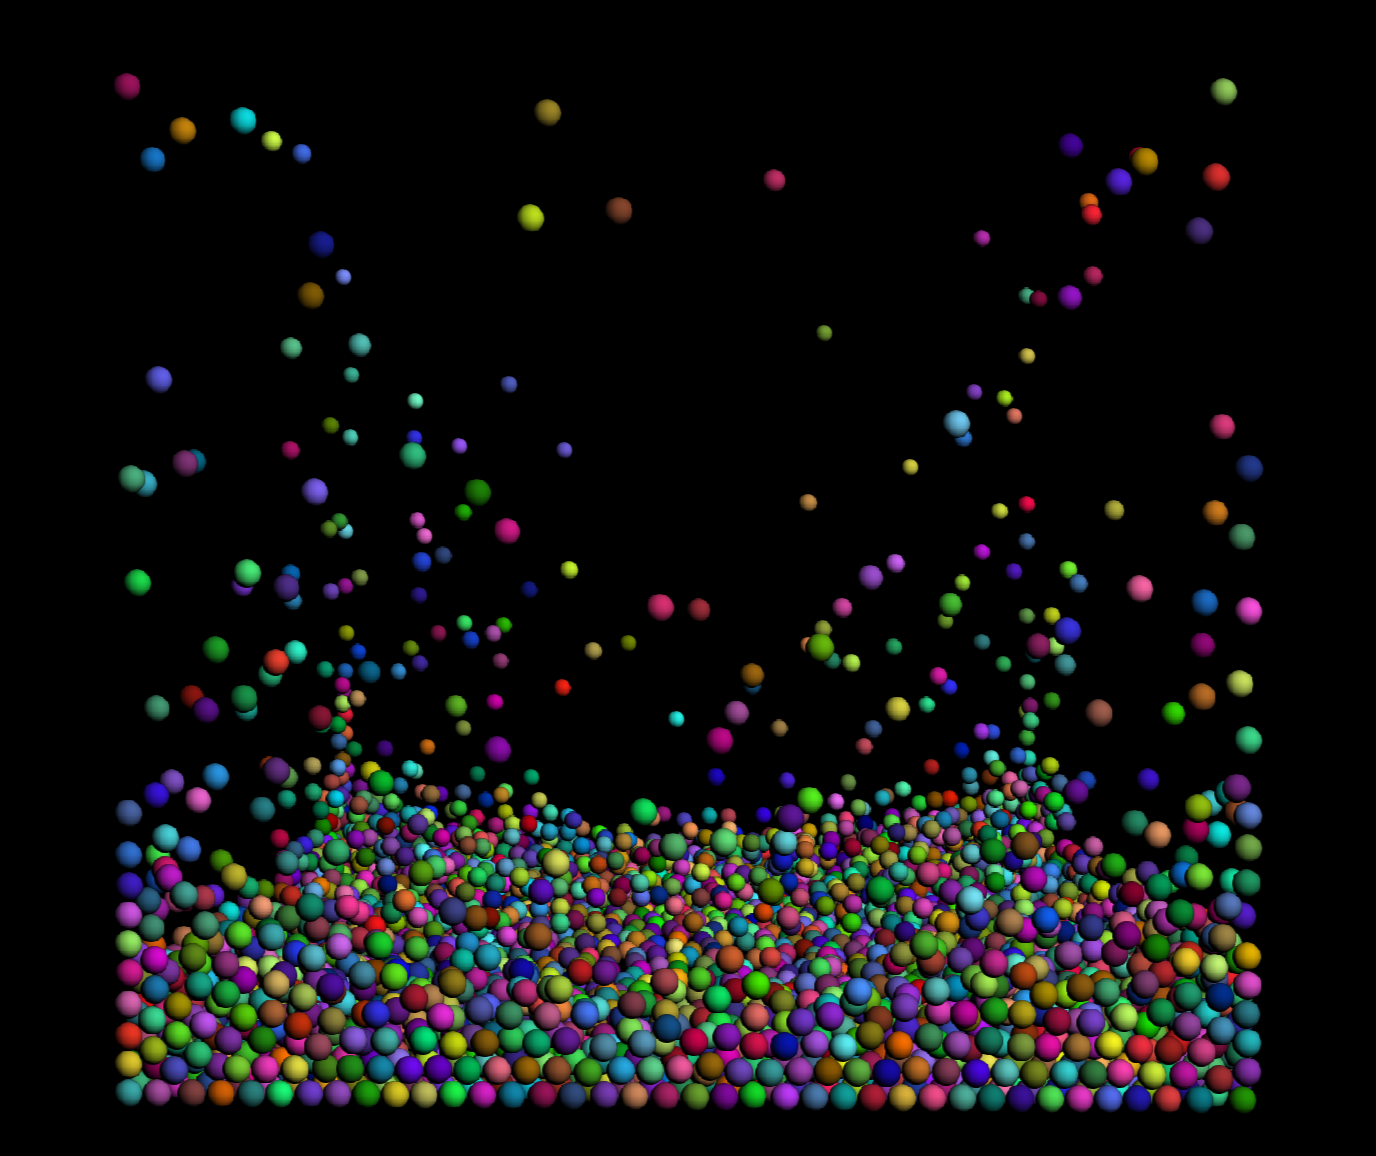
\includegraphics[scale=0.20]{figures/simulation.png}
  \captionsetup{justification=centering}
  \captionsetup{format=hang}
  \singlespace
  \caption{Simulation involving 4,096 particles. The box is invisible.}
\end{figure}

%  Starting Paragraph One
\indent\indent 
The main simulation consists of 4,096 identical particles, each having a radius of 0.4 units and a mass of 1 unit. The particles are initially arranged in a $16 \times 16 \times 16$ grid, evenly spaced within the center of a $32 \times 32 \times 32$ box. Each particle is assigned a randomized velocity ranging from 0.0 to 1.0 units per second in any direction, and the acceleration due to gravity is set at 10 units per second squared. To minimize post-collision-resolution error, the system operates at a frequency of 600 steps per second.

%___________________________________________
% Subheading 1 (remove/add as needed)
\vspace{-0.4em} % This line is added to preserve the double-spaced environment since the \section command                      adds an extra space

\section{Naive Simulation}
\indent \indent This simulation uses Gauss-Seidel position-based dynamics. 
Each simulation step involves three top level loops that iterate through each particle. Pseudocode for a single simulation step is shown below.

\begin{algorithm}
  \caption{Naive Simulation Step}\label{alg:cap}
  \begin{algorithmic}
    \For{each particle}
      \State $x_0 \gets x$
      \State $v \gets v + g \Delta t$
      \State $x \gets x + v \Delta t$
      \State Bound particle in cube
    \EndFor
    \For{$i \in$ particles}
      \For{$j \in$ particles before $i$}
        \State Resolve collision between particle $i$ and $j$
      \EndFor
    \EndFor
    \For{each particle}
      \State $v \gets \frac{x - x_0}{\Delta t}$
    \EndFor
  \end{algorithmic}
\end{algorithm}

\indent\indent The $x_0$, $x$, and $v$ represents the 
current particle's previous position, current position, and current velocity, respectively. 
$g$ represents gravity and $\Delta t$ represents the seconds per step. 
The second top-level loop resolve collisions betweeen particles
and makes the entire simulation step an $O(N^2)$ process where $N$ is the number of particles.

\section{Spatial Grid Simulation}

\begin{figure}[H]
\centering
  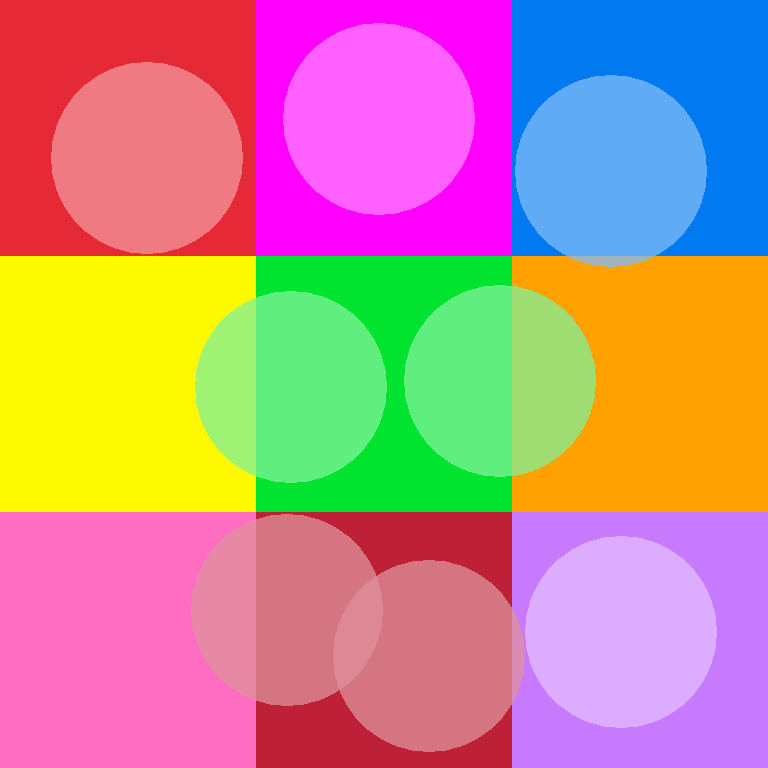
\includegraphics[scale=0.20]{figures/grid.png}
  \captionsetup{justification=centering}
  \captionsetup{format=hang}
  \singlespace
  \caption{Simulation involving 4,096 particles. The box is invisible.}
\end{figure}

\indent\indent This simulation speeds up collision detection over
the naive simulation by the usage of spatial grid, a spatial 
structure that maps the floor of the position of
each particle to the index of the particle. The spatial grid is
a three-dimensional array of linked list of indices whose dimensions
are identical to the world box. Each linked list of this grid will 
be referred to as tile for the rest of this paper. Pseudocode for a 
single simulation step is shown below.

\begin{algorithm}
  \caption{Spatial Grid Simulation Step}\label{alg:cap}
  \begin{algorithmic}
    \For{each particle}
      \State $x_0 \gets x$
      \State $v \gets v + g \Delta t$
      \State $x \gets x + v \Delta t$
      \State Bound particle in cube
    \EndFor
    \State Clear $G$
    \For{each particle}
      \State $i, j, k \gets \lfloor x \rfloor$
      \State append particle index to $G_{ijk}$
    \EndFor
    \For{$i \in$ particles}
      \For{$j \in$ particles in current and adjacent tiles}
        \State Resolve collision between particle $i$ and $j$
      \EndFor
    \EndFor
    \For{each particle}
      \State $v \gets \frac{x - x_0}{\Delta t}$
    \EndFor
  \end{algorithmic}
\end{algorithm}

\indent \indent $G$ represents the grid, and all the other
input variables are from the naive algorithm.
In the second top-level loop, the spatial grid is constructed.
In the third top-level loop, instead of looking at every
particle that comes before the current one, only the particles
in the current and adjacent tiles are looked at. 
Note, the current tile is the tile the current particle belongs to.

This is possible because each particle is smaller than a tile
and only moves a little each frame. In the average and
best case scenario $O(N)$, 
Unlike the
naive simulation, the simulation step is $O(N)$, greatly improving
performance.

\section{Edge Coloring Simulation}
This simulation speeds up collision detection ove
involves treating the grid as graph.
The tiles of the grid are treated as vertices of the graph,
and adjacent pair of tiles are treated as the edges. 
Note, that tiles are considered self-adjacent, that is an edge
is formed by tile to itself. Each tile is connected to
27 other tiles, so an edge coloring requires 27 colors.
Since the form of the graph is complile time constant,
no memory is used create the edge sets for each color. 
Instead for each step 


\vspace{-0.4em} % This line is added to preserve the double-spaced environment since the \section command                      adds an extra space

% THIS LINE ADDS THE FIRST ORDER SUBHEADING (SUBHEADING 1) TO THE TABLE OF CONTENTS (REMOVE/ADD AS NEEDED)


%%%%%%%%%%%%%%%%%%%%%%%%%%%%%%%%%%%%%%%%%%%%%%%%%%%%%%%%%%%%%%%%%%%%%%%%%%%%
%
%  Template code for the Undergraduate Research Scholars thesis program starting, updated by Undergraduate Research Scholars program staff. Version 6.0. Last Updated: Fall 2024
%  Modified by Tawfik Hussein from the template code for TAMU Theses and Dissertations starting Spring 2018, authored by Sean Zachary Roberson. Version 3.17.09.
%
%
%%%%%%%%%%%%%%%%%%%%%%%%%%%%%%%%%%%%%%%%%%%%%%%%%%%%%%%%%%%%%%%%%%%%%%%%%%%%%%%
%%%%%%%%%%%%%%%%%%%%%%%%%%%%%%%%%%%%%%%%%%%%%%%%%%%%%%%%%%%%%%%%%%%%%%%%%%%%%%%
%%                           SECTION III: RESULTS
%%%%%%%%%%%%%%%%%%%%%%%%%%%%%%%%%%%%%%%%%%%%%%%%%%%%%%%%%%%%%%%%%%%%%%%%%%%%%%%

%_________________(0)______________
% Do not modify. This is the page heading

% THIS LINE PUTS "CHAPTER III RESULTS" AT THE TOP OF THE PAGE, BOLD-FACED AND 14-PT
\chapter{RESULTS}

\counterwithout{table}{chapter} % Prevents the table count from resetting in each chapter

%________________(1)_________________
% Modifications needed!

% THIS IS THE SECTION WHERE YOU TYPE IN THE TEXT RELATED TO YOUR RESULTS. NOTICE THE DOUBLE \indent COMMAND THAT PROPERLY INDENTS THE BEGINNING OF EACH PARAGRAPH

% Starting Paragraph One
\indent \indent Paragraph one starts here. If you want to break up your paragraphs into more sections, you can use first order, second order or third order subheadings. 
\\
\indent \indent Feel free to add more Chapters as necessary, but don’t forget to include the Chapter Headings as seen at the top of this page. Also remember that all new Chapters should begin at the top of their own pages and be included in the Table of Contents.
%
%___________________________________________
% Subheading 1 (remove/add as needed)
\vspace{-0.4em} % This line is added to preserve the double-spaced environment since the \section command                      adds an extra space 
\section{Results Subheading 1 (remove/add as needed)}
\vspace{-0.4em} % This line is added to preserve the double-spaced environment since the \section command                      adds an extra space

\indent \indent If you need to enumerate some ideas, the \textit{enumerate} environment can be used to generate an ordered list. The following example illustrates how to do so:
\vspace{-2em}
\begin{singlespace}
\begin{enumerate}
\item This is item number one.
\item This is item number two.
\item This is item number three.
\item This is item number four.
\end{enumerate}
\end{singlespace}
\vspace{-1em}
%
%
%___________________________________________
% Subheading 2 (remove/add as needed)

\section{Results Subheading 2 (remove/add as needed)}
\vspace{-0.4em} % This line is added to preserve the double-spaced environment since the \section command                      adds an extra space

% THIS LINE ADDS ANOTHER FIRST ORDER SUBHEADING (SUBHEADING 2) TO THE TABLE OF CONTENTS (REMOVE/ADD AS NEEDED)
%\addcontentsline{toc}{section}{\hspace{4.2em} \textcolor{red}{Subheading 2 (remove/add as needed)}}

\indent\indent Here is another example of a figure in this section ({\bf Figure 2}). Make sure you always reference your figures in the body text. 

\begin{figure}[h!]
	\centering
	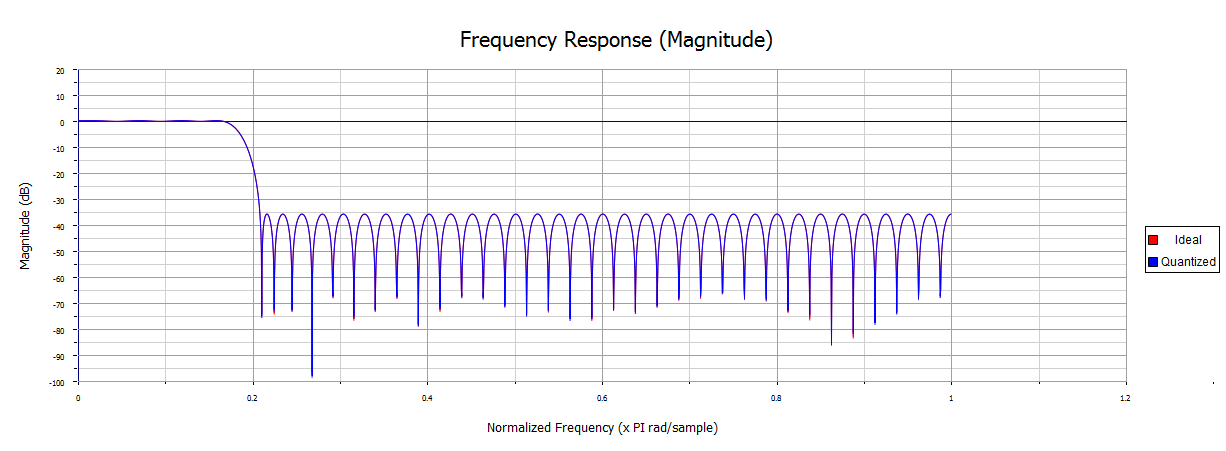
\includegraphics[width = 6.0in]{LowPass_Filter_Design.png}
	\caption{A low pass filter design.}
\end{figure}


 





%%%%%%%%%%%%%%%%%%%%%%%%%%%%%%%%%%%%%%%%%%%%%%%%%%%%%%%%%%%%%%%%%%%%%%%%%%%%
%
%  Template code for the Undergraduate Research Scholars thesis program starting, updated by Undergraduate Research Scholars program staff. Version 6.0. Last Updated: Fall 2024
%  Modified by Tawfik Hussein from the template code for TAMU Theses and Dissertations starting Spring 2018, authored by Sean Zachary Roberson. Version 3.17.09.
%
%
%%%%%%%%%%%%%%%%%%%%%%%%%%%%%%%%%%%%%%%%%%%%%%%%%%%%%%%%%%%%%%%%%%%%%%%%%%%%%%%
%%%%%%%%%%%%%%%%%%%%%%%%%%%%%%%%%%%%%%%%%%%%%%%%%%%%%%%%%%%%%%%%%%%%%%%%%%%
%%                           SECTION IV: CONCLUSION
%%%%%%%%%%%%%%%%%%%%%%%%%%%%%%%%%%%%%%%%%%%%%%%%%%%%%%%%%%%%%%%%%%%%%%%%%%%
%________(0)__________
% Do not modify. This is the page heading.

% THIS LINE PUTS "CHAPTER IV CONCLUSION" AT THE TOP OF THE PAGE, BOLD-FACED AND 14-PT
\chapter{CONCLUSION}

% THIS LINE ADDS THE CONCLUSION TO THE TABLE OF CONTENTS
%\addcontentsline{toc}{chapter}{\vspace{1.0em}\hspace{1.0em} IV.\hspace{2em}CONCLUSION} 


%__________(1)_________
% Modification Needed!

% THIS IS THE SECTION WHERE YOU TYPE IN THE TEXT RELATED TO YOUR CONCLUSION. NOTICE THE DOUBLE \indent COMMAND THAT PROPERLY INDENTS THE BEGINNING OF EACH PARAGRAPH

\section{Conclusion Subheading}

\indent \indent Paragraph one starts here. If you want to break up your paragraphs into more sections, you can use first order, second order or third order subheadings.

%___________________(X)__________________________
% Optional section. Either keep or delete depending on your needs.

% THIS SECTION IS JUST AN EXAMPLE OF HOW TO ADD FIRST ORDER SUBHEADINGS TO THE TABLE OF CONTENTS. IF YOU DO HAPPEN TO HAVE/NEED MORE SUBHEADINGS IN THIS SECTION, MAKE SURE YOU ADD THE LINE OF CODE BELOW (PER SUBHEADING) TO THE APPROPRIATE SECTION IN YOUR CODE, SIMILAR TO HOW IT IS DEMONSTRATED IN THE METHODS AND RESULTS SECTIONS.

% \section{Another Subheading}






% The next line is the format for inserting new sections.
% Replace the name "newsection"  with the name of your
% new section file.
% \include{data/newsection}

% fix spacing in bibliography, if any...
%%%%%%%%%%%%%%%%%%%%%%%%%%%%%%%%%%%%%%%%%%%%%%%%%%%%%%%%%%%%%

\let\oldbibitem\bibitem
\renewcommand{\bibitem}{\setlength{\itemsep}{0pt}\oldbibitem}
\renewcommand{\bibitem}{\vspace{1em}\setstretch{1.0}\oldbibitem}

%%%%%%%%%%%%%%%%%%%%%%%%%%%%%%%%%%%%%%%%%%%%%%%%%%%%%%%%%%%%%%%
% The bibliography style declared is the IEEE format. 

\bibliographystyle{ieeetr}

\phantomsection
\addcontentsline{toc}{chapter}{REFERENCES}

\renewcommand{\bibname}{{\large\ \bf \textcolor{black}{REFERENCES}}}

%This file is a .bib database that contains the sources.
%This removes the dependency on the previous file
%bibliography.tex.

\bibliography{data/12-References}


% This next line includes appendices. The file
% appendix.tex contains commands pointing to
% the appendix files; be sure to change these
% pointers if you end up changing the filenames.
% Leave this commented if you will not need
% appendix material.
%%%%%%%%%%%%%%%%%%%%%%%%%%%%%%%%%%%%%%%%%%%%%%%%%%%%%%%%%%%%%%%%%%%%%%%%%%%%%
%
%  Template code for the Undergraduate Research Scholars thesis program starting, updated by Undergraduate Research Scholars program staff. Version 6.0. Last Updated: Fall 2024
%  Modified by Tawfik Hussein from the template code for TAMU Theses and Dissertations starting Spring 2018, authored by Sean Zachary Roberson. Version 3.17.09.
%
%
%%%%%%%%%%%%%%%%%%%%%%%%%%%%%%%%%%%%%%%%%%%%%%%%%%%%%%%%%%%%%%%%%%%%%%%%%%%%%%%

%%%%%%%%%%%%%%%%%%%%%%%%%%%%%%%%%%%%%%%%%%%%%%%%%%%%%%%%%%%%%%%%%%%%%%%%%%%
%%                           APPENDIX 
%%%%%%%%%%%%%%%%%%%%%%%%%%%%%%%%%%%%%%%%%%%%%%%%%%%%%%%%%%%%%%%%%%%%%%%%%%%

% The Appendix section is optional, must be placed directly after the references section, can be a collection of large data sets, images, and/or tables tghat would interrupt a significant portion of your writing. It can be a single Appendix (label as Appendix: Title) or it can include multiple Appendices (label as Appendix A: Title, Appendix B: Title, etc). Label figures, tables, and equations consecutively starting with A.1, A.2, etc. For additional Appendices (B, C, etc.), label figures, tables, and equations as B.1, B.2, etc. It can also be as many pages as needed.

%_________(0)____________

% Do not modify this section. This ensures proper formatting of the appendix tables, equations, and figures.

\phantomsection

\chapter*{\large\bf APPENDIX: TITLE}
\addcontentsline{toc}{chapter}{APPENDIX: TITLE} 

% These two lines reset the counter for figures and adds an "A" before each figure number (i.e, Figure A.1)

\renewcommand{\thefigure}{A.\arabic{figure}}
\setcounter{figure}{0}

% These two lines reset the counter for tables and adds an "A" before each figure number (i.e, tables A.1)
\renewcommand{\thetable}{A.\arabic{table}}
\setcounter{table}{0}

\renewcommand{\theequation}{A.\arabic{equation}}
\setcounter{equation}{0}

%___________(1)____________
% Modifications needed! 

% [INSTRUCTIONS FOR REQUIRED ACKNOWLEDGEMENTS PAGE.]

%The Appendix section: 
%\begin{itemize}
%  \item Is optional
%  \item Must be placed directly after the References section
%  \item Can be a collection of large data sets, images, and/or tables that would interrupt a significant portion of your writing
%  \item Can be a single Appendix (label as Appendix: Title)
%  \item Can include multiple Appendices (label as Appendix A: Title, Appendix B: Title, etc.)
%  \item Label figures, tables, and equations consecutively starting with A.1, A.2, etc. For additional Appendices (B, C, etc.), label figures, tables, and equations as B.1, B.2, etc.
%  \item Can be as many pages as needed
%\end{itemize}

%____________(2)_________________
% MODIFY THE SAMPLE APPENDIX PAGE. INCLUDES EXAMPLE FIGURES WITH PROPER CAPTION LABELLING AND NUMBERING. 
[Type content here.]

\begin{table}[htp]
    \centering
    \caption{Call this table A.1.}
    \label{tab1}
  	\begin{tabular}{|l|l|l|l|}  % Each "l" corresponds to a column in the table. Hence, the total number of "l"
	                            % corresponds to the number of columns your table will have.
		\hline
		\bf{Heading 1} & \bf{Heading 2} & \bf{Heading 3} & \bf{Heading 4} \\ \hline
		Content example. & Content example. & Content example. & Content example. \\ \hline
		Content example. & Content example. & Content example. & Content example. \\ \hline
    \end{tabular}
\end{table}

\begin{figure}[H]
\centering    % This centers it
	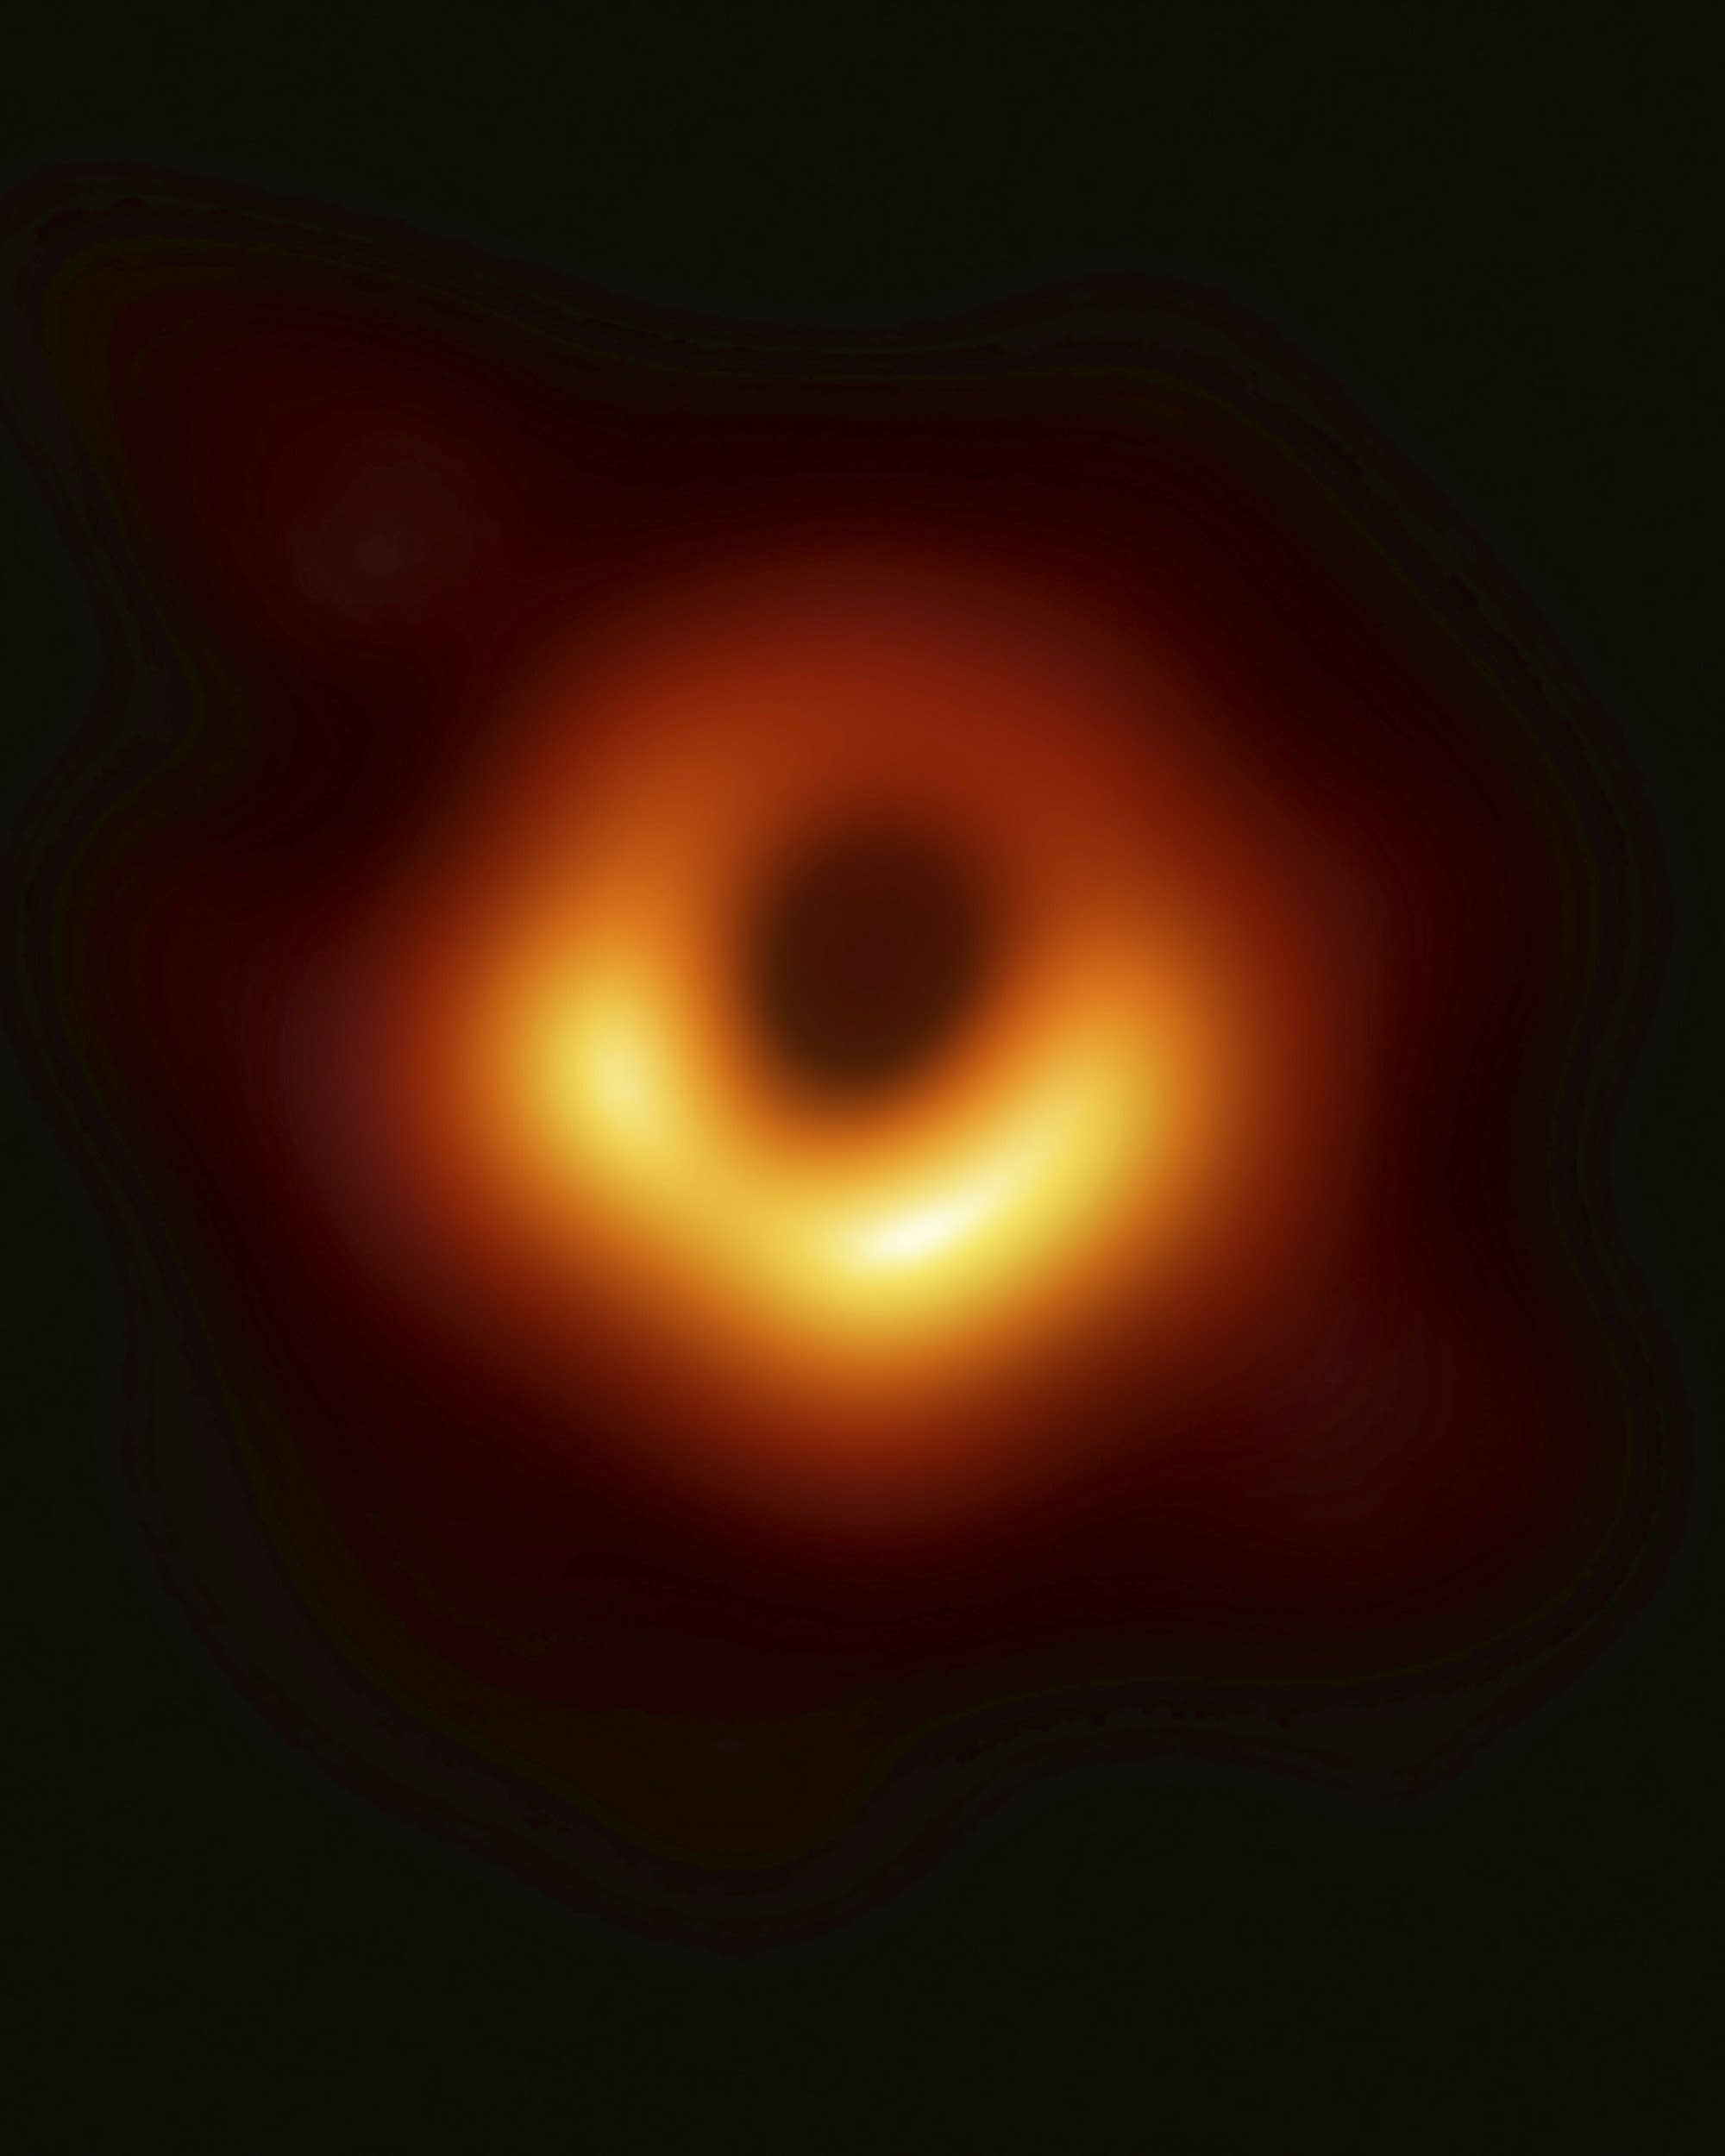
\includegraphics[scale=0.10]{figures/blackhole.jpg}
	\captionsetup{justification=centering}
	\captionsetup{format=hang}
        \singlespace
	\caption{The first recorded image of a black hole}    % This is the caption of the figure
%\label{figa2}
\end{figure}

\begin{equation} \label{Equ.A.1}
R_{\mu \nu} - {\frac{1}{2}}g_{\mu \nu}\,R + g_{\mu \nu} \Lambda = 
 {\frac{8 \pi G}{c^4}} T_{\mu \nu}
\end{equation}

\end{document}
